\chapter{Planificación}\label{chap:planif}
La planificación de un proyecto es fundamental para su correcto funcionamiento y desarrollo,
dentro de los plazos y costes establecidos. En este apartado se detallan las tareas que se
llevarán a cabo en el proyecto, así como los recursos necesarios y los plazos de ejecución.

\section{Partes interesadas (stakeholders)}\label{sec:stakeholders}
Las partes interesadas en el proyecto son aquellas personas o entidades que tienen un interés
en el mismo, ya sea porque se ven afectadas por el resultado del proyecto, o porque tienen
algún tipo de interés en el mismo. Las partes interesadas en este proyecto son las siguientes:

\begin{enumerate}
	\item \textbf{Okticket}: la empresa es la principal parte interesada en el proyecto, ya que
		es la que se beneficiará directamente de los resultados del mismo, así como de las
		oportunidades de negocio que se abren con la explotación de los datos.
		\begin{itemize}
			\item \textbf{Equipo de desarrollo}: el equipo de desarrollo es otra parte interesada en el
				proyecto, ya que son los encargados de llevar a cabo la implementación del sistema y
				de garantizar su correcto funcionamiento.
			\item \textbf{Equipo de soporte}: el sistema planteado ahorraría tiempo al equipo de
				soporte, ya que les permitiría analizar los datos de forma más eficiente e identificar
				problemas antes de que tener que resolver las peticiones de los clientes afectados.
		\end{itemize}
	\item \textbf{Clientes}: los clientes de la empresa también son partes interesadas, puesto
		que se beneficiarán de los nuevos servicios que se ofrecen, como los dashboards de
		negocio que se han descrito anteriormente.
	\item \textbf{Investigador y desarrollador:} el desarrollador del proyecto tiene la oportunidad de
		aplicar los conocimientos adquiridos en el desarrollo de un proyecto real, y de adquirir
		nuevos conocimientos en el proceso.
\end{enumerate}

\section{Metodología}\label{sec:metodología}
\subsection{Scrum}\label{subsec:scrum}
Para la planificación del proyecto se ha escogido \textit{Scrum}, una metodología ``ágil'' que se
basa en la realización de iteraciones cortas y en la adaptación a los cambios. La metodología
\textit{Scrum} se estructura en \textit{sprints} (iteraciones cortas de una duración fija),
en las que se llevan a cabo una serie de tareas que se han planificado previamente.

El primer paso de la metodología \textit{Scrum} es la creación de un \textit{product backlog},
una lista ordenada de las tareas a realizar durante el desarrollo del producto, a partir de los
requisitos del sistema, que a su vez son una versión refinada de los requisitos iniciales del
proyecto. A partir de este \textit{product backlog} se planifican las tareas que se llevarán
a cabo en cada \textit{sprint}, de manera que sea posible cumplir con los objetivos del proyecto
en el tiempo establecido.

\subsection{Visualización de la planificación}\label{subsec:visual_planif}
Para la visualización de la planificación se ha utilizado la herramienta de gestión de proyectos
de \textit{GitHub}, que permite múltiples visualizaciones de tareas e \textit{issues} en tableros
separados.

\begin{itemize}
	\item Se utiliza un tablero de \textit{requisitos} al estilo \textit{Kanban} para visualizar
		los requisitos del proyecto y su estado, siguiendo con la metodología \textit{Scrum}.
	\item Se utiliza un \textit{roadmap} de tareas, donde se visualizan las tareas y los hitos
		del proyecto, así como su estado y sus fechas límite.
\end{itemize}

\begin{minipage}{\linewidth}
	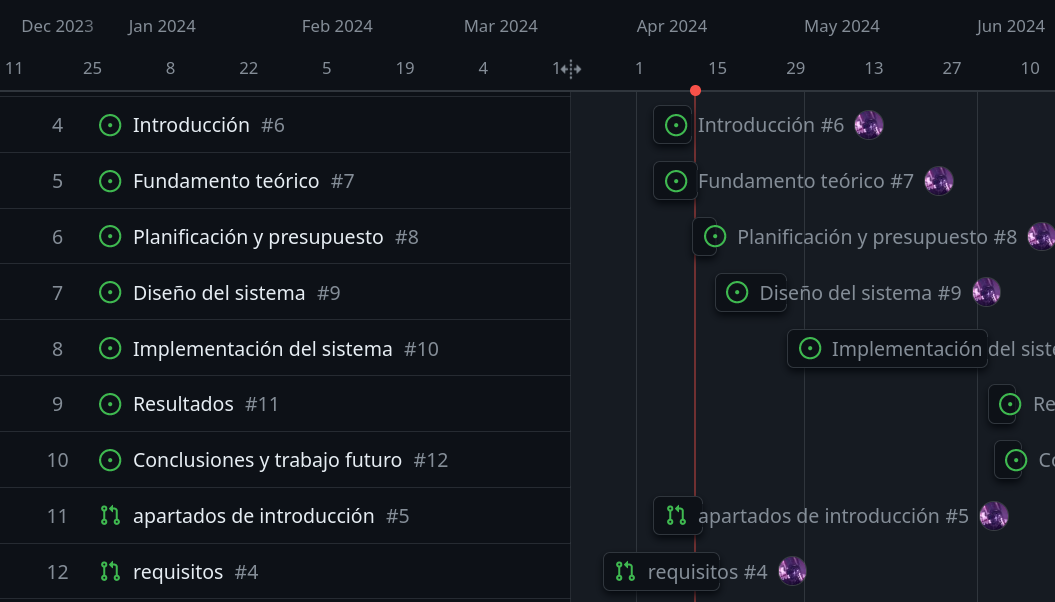
\includegraphics[width=0.95\textwidth]{roadmap.png}
	\captionof{figure}{Roadmap de tareas}
\end{minipage}

\subsection{Comunicación}\label{subsec:comunicación}
La comunicación con los tutores y con el equipo de desarrollo se considera fundamental para el
correcto desarrollo del proyecto. Puesto que el trabajo se desarrolla de manera presencial en
la oficina de la empresa, la comunicación con el equipo de desarrollo se realiza de manera
frecuente y directa, mientras que la comunicación con los tutores se realiza de manera remota
pero igual de frecuente, manteniendo el contacto mediante correo electrónico y Teams para
pedir revisiones e informar sobre el estado del trabajo en todo momento.

\section{Presupuesto}\label{sec:presupuesto}
